\documentclass{article}
\usepackage[margin=1in]{geometry} 
\usepackage{amsmath,amsthm,amssymb,amsfonts, fancyhdr, color, comment, graphicx, environ}
\usepackage{xcolor}
\usepackage{mdframed}
\usepackage[shortlabels]{enumitem}
\usepackage{indentfirst}
\usepackage{hyperref}
\hypersetup{
    colorlinks=true,
    linkcolor=blue,
    filecolor=magenta,      
    urlcolor=blue,
}
\usepackage{pgfplots}
\pgfplotsset{width=10cm,compat=1.9}
\pgfplotsset{compat=1.17}
\usepackage{tikz}
\usepackage{caption}

\setlength{\parindent}{0pt}


%for headers 
\pagestyle{fancy}
\fancyhf{} % for header/footer

\lhead{Creel}
\rhead{ENV 795 - Nature as Capital}
\chead{\textbf{Utility}}

\title{Section Two - Aggregating Utility}
\author{Andie Creel for Nature as Capital}
\date{February 13th, 2023}

\begin{document}
\maketitle

\section{Utility Functions}

\subsection{Overview}

Individuals consume bundles of goods and gain welfare from the act of consuming. The utility function assigns a numerical representation of welfare to every bundle of goods so that we can order which bundles are better than others. The higher an individual's utility level, the better off that individual is. \\

Do not get hung up on the word \textit{consume}. Everyone here knows that visiting parks or seeing a grizzly bear (from afar) or knowing that an endangered species still exists can contribute to an individual's welfare. I consider these experiences a \textit{good} that can be \textit{consumed} and therefore we can use utility functions to assign numerical representations of welfare to these experiences.\\

There are three common assumptions about the behavior of utility functions: 
    \begin{enumerate}
    \item \textbf{Increasing}: The more goods I consume, the higher my utility level. You may also hear the term \textit{monotonically increasing}. For our purposes, you may just think of it as increasing. "Goods are good."\\
    \newline
    In math: Let $A$ and $B$ be bundles of goods: $A \succ B \implies U(A) > U(B)$. 
    \item \textbf{Concave}: Diminishing marginal returns -- the marginal utility I get from the first slice of pie is greater than the marginal utility I get from the 7th.\\
    \newline
    In math: If $A \succ B \implies  U'(A) < U'(B)$
    \item \textbf{Continuous}: The utility function is a continuous function. This less about imposing a behavior assumption on the utility function to model people's behavior and more about the math being nice. \\
    \newline
    In math: $\lim_{x \rightarrow c} U(x) = U(c)$
    
    \end{enumerate}

\subsection{A note on "bundles"}
We've been talking about "bundles" of goods. A bundle established the quantity of each good you're consuming. For example, say you consume clothes and food. Bundle $A$ is 4 clothes and 5 foods. Bundle $B$ is 6 clothes and 5 foods. I know you prefer bundle $B$ to bundle $A$, because there are more clothes and the same about of food. Now consider bundle $C$, which is 5 clothes and 4 foods. Without a utility function, I don't know if you prefer $A$ or $B$.\\

\begin{figure}[htp]
    \centering
    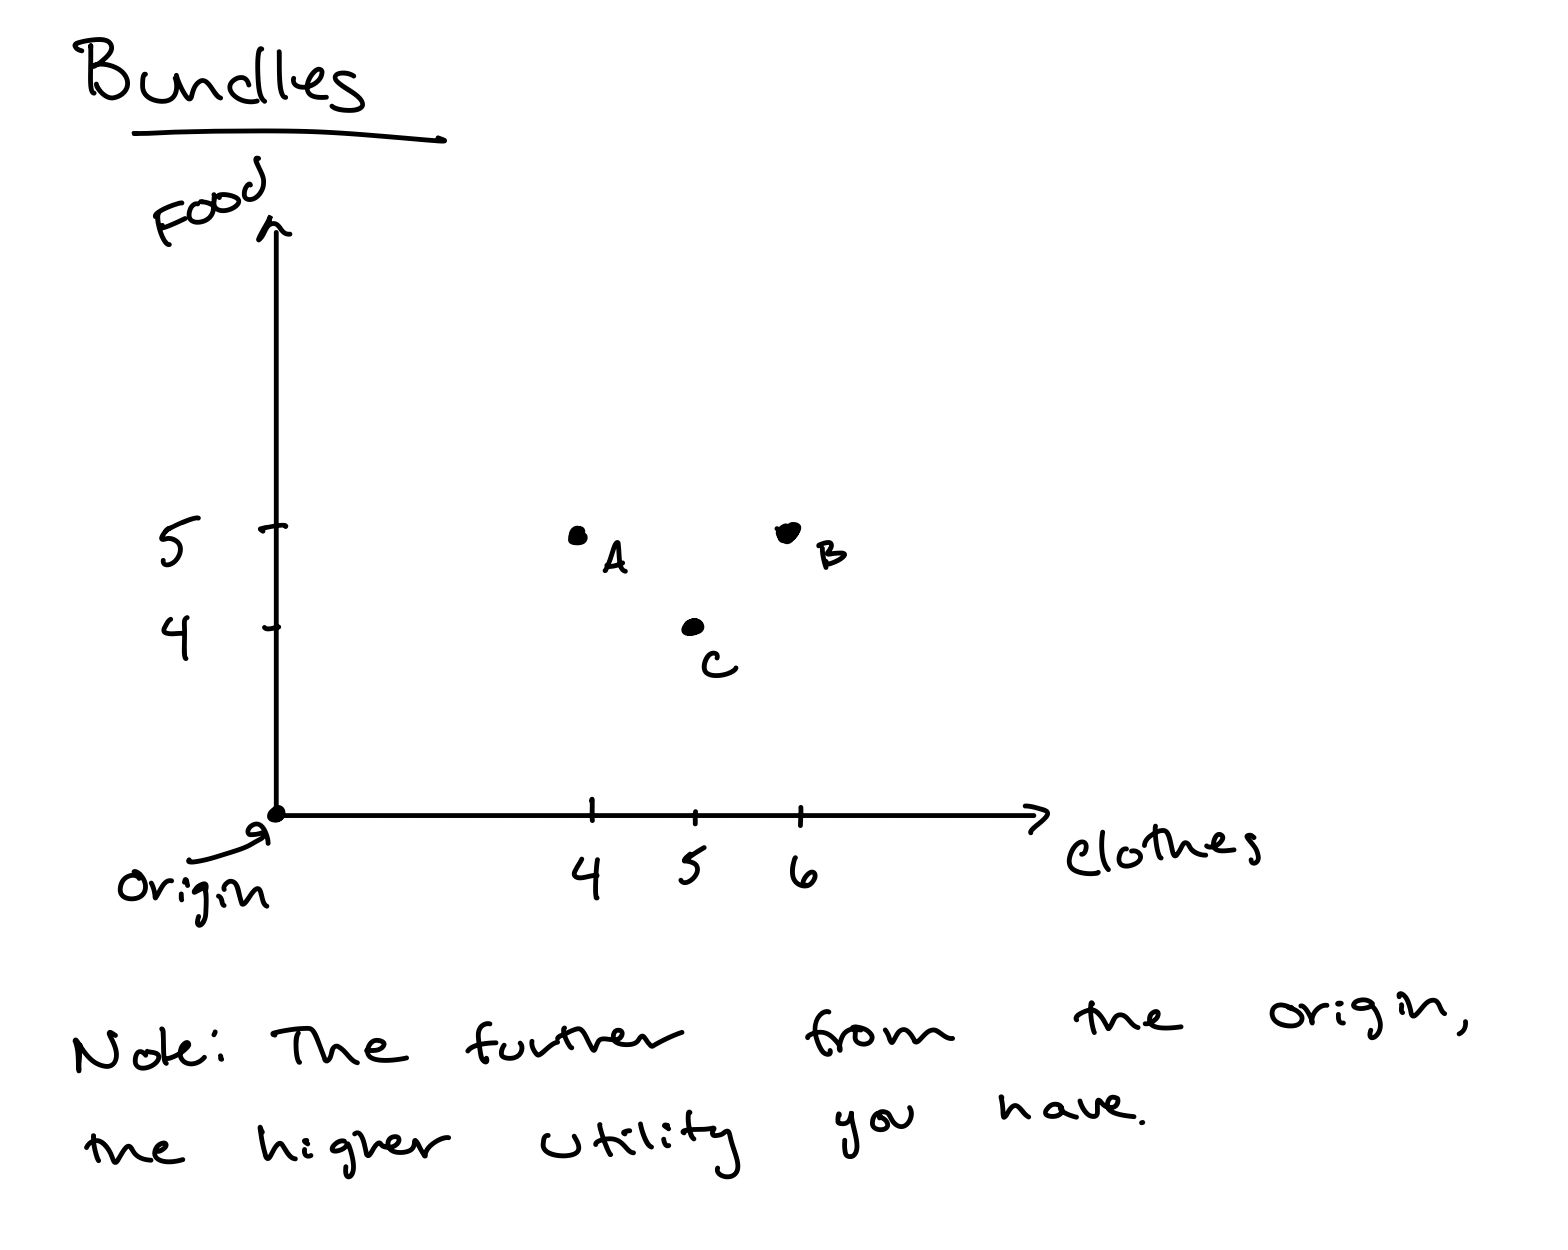
\includegraphics[width=7cm]{Screen Shot 2023-02-13 at 3.40.02 PM.png}
    \caption{}
\end{figure}


\textbf{Notation:} Utility functions assign numeric values of welfare to bundles of goods. In this case our bundle is clothes and food, $U(clothes, food)$. We could also call clothes $X$ and food $Y$, and write our utility function as $U(X,Y)$. 
 
\subsection{Examples of Utility Functions}
There are two functional forms of utility functions that meet the three common assumptions above that are used frequently in economic models. \\

Notation: Let $C$ denote a bundle, and a bundle is made up of $X$ and $Y$, $C = \{X, Y\}.$\\

\textbf{Cobb-Douglas}:

$$U(C) = U(X,Y) = X^\alpha Y^\beta$$

Often, you'll see a log transformation of Cobb-Douglas Utility. Log transformations are useful because they will not change the order of which bundles we prefer the most.
$$ln(U(C)) = \alpha ln(X) + \beta ln(Y)$$

\textbf{Constant Relative Risk Aversion}:

$$U(C) = \frac{C^{1-\eta} - 1}{1 - \eta}$$

Where $\eta$ can be interpreted as the coefficient of relative risk aversion AND defines the intertemporal elasticity of substitution (aka consumption elasticity of marginal utility), $\frac{1}{\eta}$. \\

\begin{figure}[htp]
    \centering
    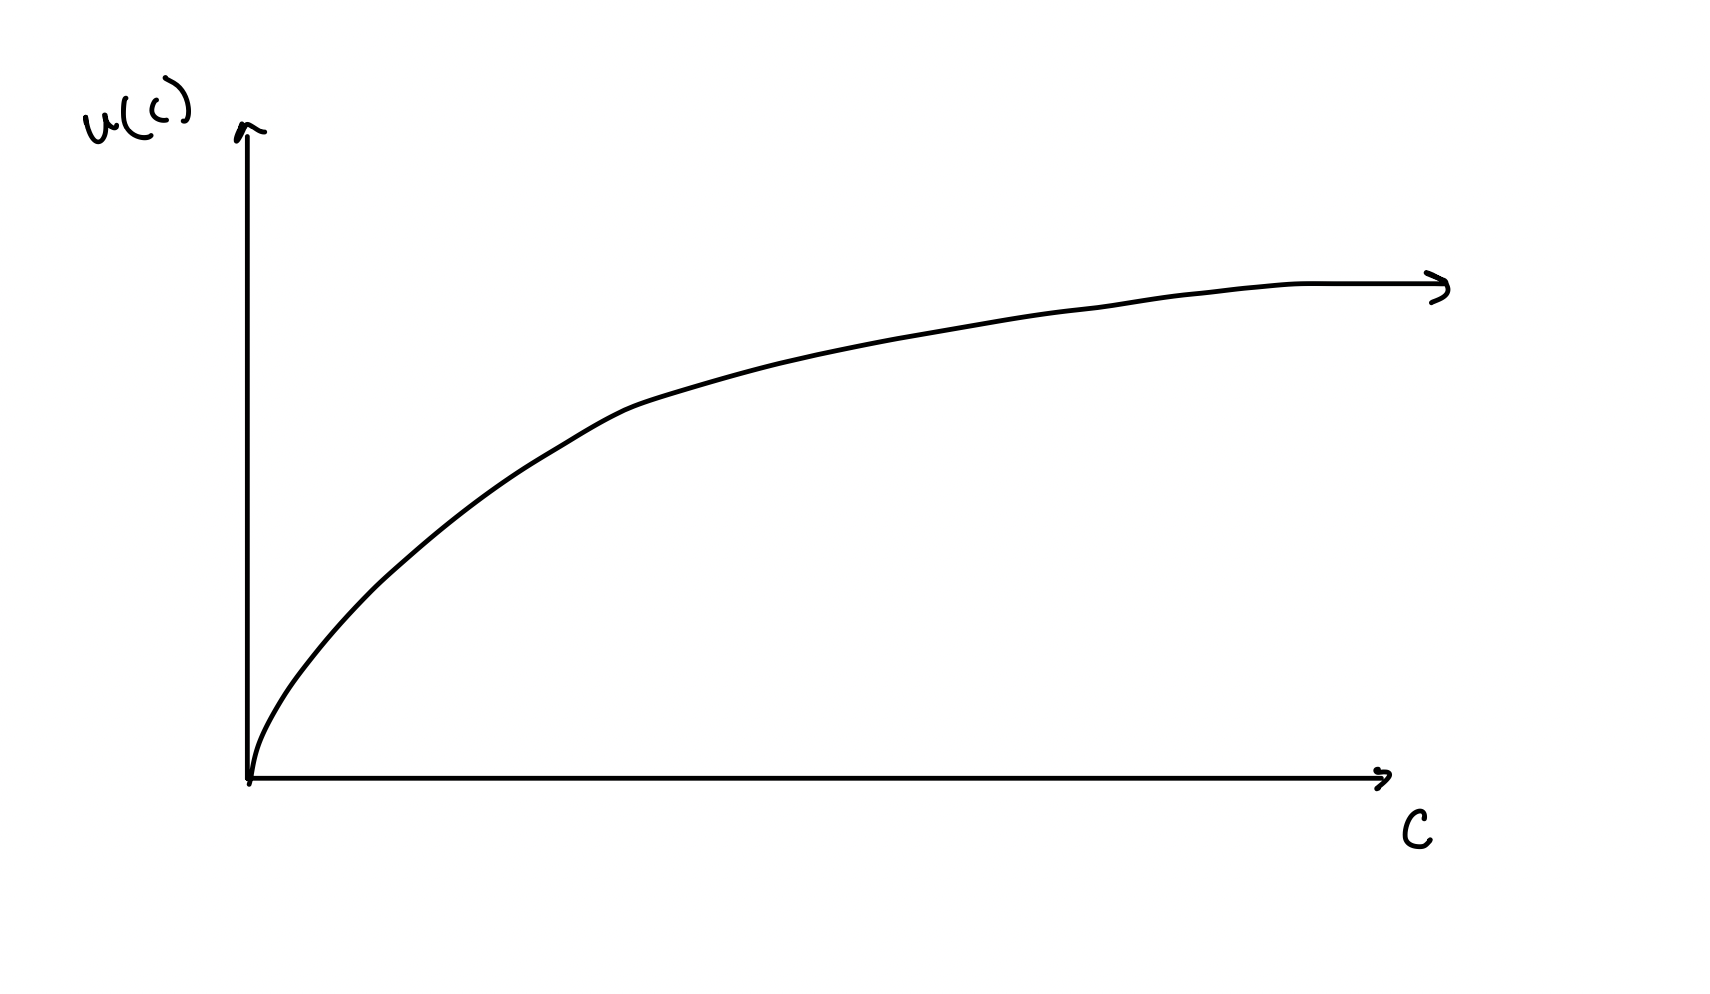
\includegraphics[width=7cm]{Screen Shot 2023-02-13 at 3.40.54 PM.png}
    \caption{}
\end{figure}


\section{Summing Utility Through Time -- Discounting}
Discount rates are what let us sum utility through time OR consider whether a project that provides benefit in the future is worth investing in today. 

\begin{figure}[htp]
    \centering
    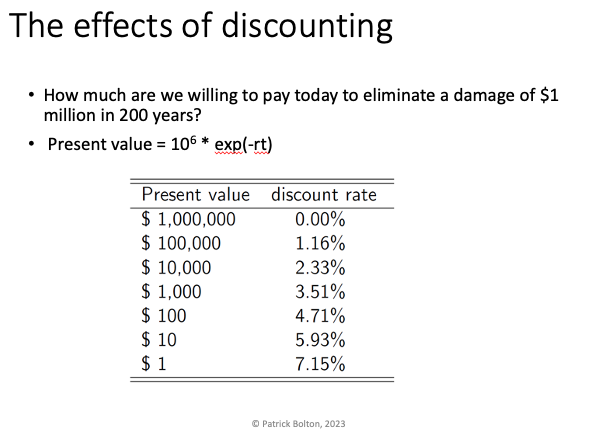
\includegraphics[width=12cm]{Screen Shot 2023-02-13 at 3.18.01 PM.png}
    \caption{Patrick Heal's presentation to Climate Finance in 2023}
\end{figure}

\subsection{Continuous Time}
Consider an infrastructure project that will provide $v$ units of benefit \textit{every instant} from now until time period $T$. The infrastructure project would cost \$100 today, and you want to know if the benefits are greater than the costs. 

$$B = \int_0^T e^{-rt} U(C_t) dt  = \int_0^T e^{-rt} v dt$$
where $exp(-rt)$ is our discount factor. And $e^{-rt} v$ is the present value of the benefit in time period $t$. \\

If $B > 100$, then the project is profitable.

\subsection{Discrete Time}

Now consider an infrastructure project that will provide $v$ units of benefit \textbf{every year} from now until time period T. 

$$B = \sum_0^T (\frac{1}{1+r})^t * U(C_t) dt  = \sum_0^T (\frac{1}{1+r})^t * v dt$$

\section{Summing Utility Across Individuals -- Negishi Weights}
Discussion: if you are interested in any wealth redistribution policy, you cannot use Negishi weights to model it because they hold the wealth distribution constant. 





\end{document}
